\addchapheadtotoc

\chapter{Findings}
The Gross-Pitaevskii equation exhibits numerical chaos when an initial turbulent state evolves in zero potential. Chaos is seen for positive values of $g$. For positive nonlinear coupling constant $g$, the relationship between the Lyapunov exponent is seemingly linear, as shown in Figure \ref{fig:glam}. For negative $g$, there is no clear relationship. Shown in Figure \ref{fig:gline}, applying a linear regression for positive $g$ results in \begin{equation}
	\lambda(g) = \num{0.04996 \pm 0.00206} g + \num{0.0197 \pm 0.0125},
\end{equation}
with $p<0.01$ and $R^2=0.986$, indicating correlation and a high degree of fitment. 
\begin{figure}[p]
	\centering
	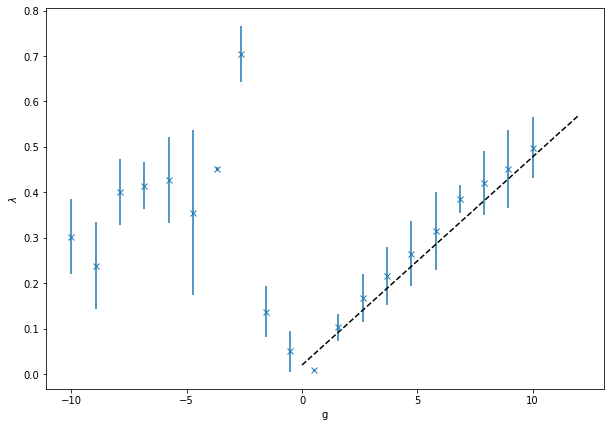
\includegraphics[width=0.7\linewidth]{chapter4/g_lam}
	\caption{The effect of $g$ on the Lyapunov exponent. Note the cross represents the mean for that sample and the error bars denote the standard deviation from $N=5$ samples.}
	\label{fig:glam}
\end{figure}

\begin{figure}[p]
	\centering
	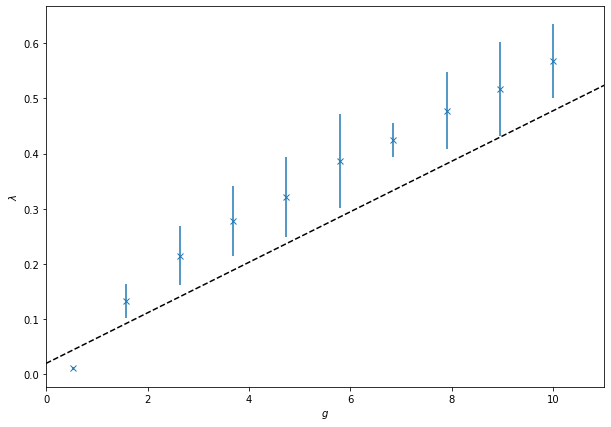
\includegraphics[width=0.7\linewidth]{chapter4/g_line}
	\caption{Linear fit on positive coupling constant $g$ versus the Lyapunov exponent.}
	\label{fig:gline}
\end{figure}



\section{Error analysis}
Several steps were taken to ensure error is minimized. First, both wavefunctions are evolved backward in time to ensure convergence to their original wavefunction. Next, we check the role of tolerances used in the solver and its effect on the Lyapunov exponent. Lastly, the role of machine precision is discussed.


\subsection{Reverse time evolution}
After each experiment, the wavefunctions are evolved backwards in time to the original time step, attempting to perfectly recover the original wavefunction, akin to the Loschmidt echo. This wavefunction is compared to the original wavefunction to ensure error in the solver is minimized by iterating over the spatial dimension and finding the difference at each point. The time-reversed wavefunction were found to be equal to the original within an absolute tolerance of \num{1e-10}. This value is beyond the tolerances of the solver, indicating recovery of the original wavefunction.


\subsubsection{Role of solver tolerances}
The Gross-Pitaevskii equation with coupling constant $g=0$ returns the Schr\"odinger equation, a linear differential equation and we should expect a Lyapunov exponent of zero. Experimentally, the Lyapunov exponent for this case was found to be zero for high-precision absolute and relative solver tolerances of \num{1e-10} and smaller. For lower-precision tolerances, the solver fails, as shown in Figure \ref{fig:tollam}. For the nonzero $g$, a solver tolerance of \num{1e-10} is then specified.

\begin{figure}[p]
	\centering
	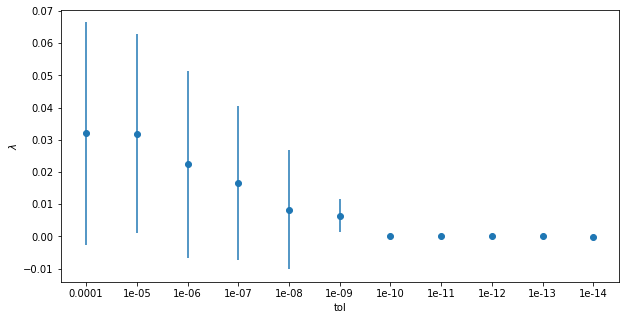
\includegraphics[width=\linewidth]{chapter4/tol_lam}
	\caption{Effect of solver tolerances on the Lyapunov exponent for the non-chaotic Schr\"odinger equation. The Lyapunov exponent is expected to return zero. For higher tolerances ($<\num{1e-10}$), the error is significantly increased indicating poor precision and solver failure.}
	\label{fig:tollam}
\end{figure}

\subsubsection{Role of machine precision and spatial derivative error}
In the simulation, NumPy is a library used for performing mathematical and matrix operations. The library relies on 64-bit floating point numbers, as specified by IEEE-754. The machine precision of floating point numbers as defined in IEEE-754 is the limiting precision on floating point numbers in the simulated Gross-Pitaevskii equation \cite{1985--ieee754}. This value is defined in the specification as \begin{equation}
	\epsilon = \num{2.22e-16}.
\end{equation}
This value must be taken into account when setting both the lattice spacing $h$ and the solver tolerances.